\chapter{Full Cross Section Data}
To be completed

\chapter{BSA Cross Check}

As an additional cross check, Bobby calculated a $DV\pi^0P$ beam spin asymmetry and compared to Andrey Kim's results. This check will not comment on any acceptance, luminosity, or virtual photon flux factor calculations, but does validate exclusive event selection criteria. By examining figure \ref{fig:bsa} we can see that agreement is reasonable, especially considering Bobby's calculation does not have sideband subtraction included.

\begin{figure}[hbt]
	\centering
	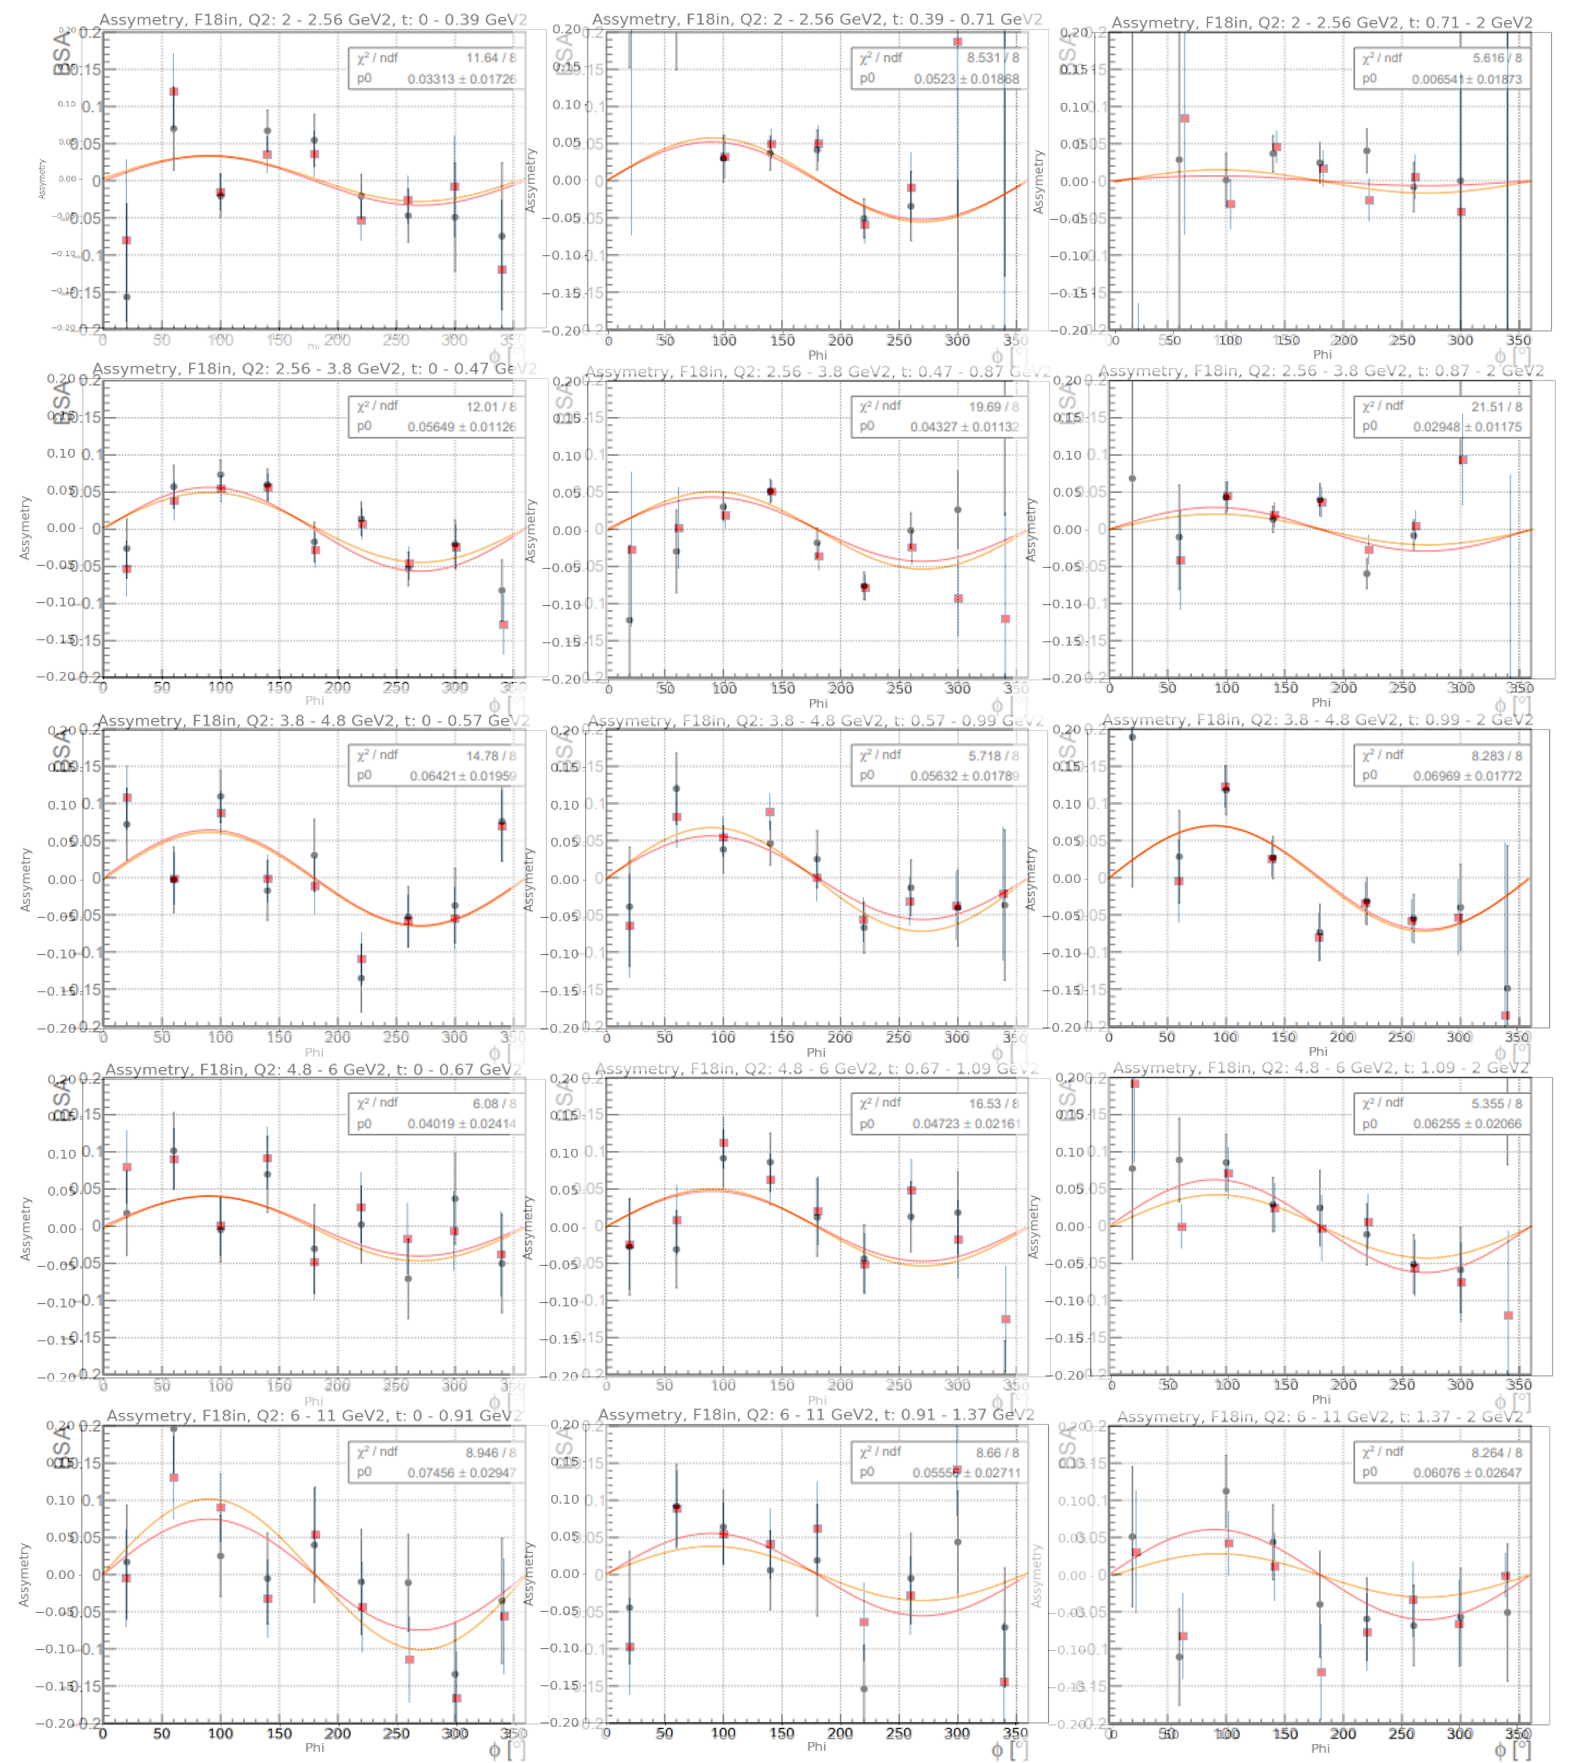
\includegraphics[width=0.75\linewidth]{Chapters/Postamble/appb_pics/BSA.png}
	
	
	\caption{BSA Cross Check Results}
	\label{fig:bsa}
\end{figure}

Fig \ref{fig:bsa} shows an overlay comparison of Andrey Kim's results (black datapoints, red fit line) and Bobby's results (red datapoints, orange fit line
\chapter{Derivation of phi math convention}


Thus:
phi = arccos( (v3l dot v3h) / (mag v3l mag v3h) ) 

phi =    \footnotesize{$\cos^{-1} \left( \frac{ \left(p_{e} \times p_{e'} \right) \cdot \left( p_{p'} \times p_{\gamma^*} \right) }{ \lVert p_{e} \times p_{e'} \rVert \: \lVert p_{p'} \times p_{\gamma^*} \rVert} \right)$}

if dot(pe cross pe', pp') is greater than 0, then do 360 - phi = phi.
If we expand the above out, we get:
-pp'x*ez*ey' + py*ez*ex' is greater than zero
which we can reduce to 
-pp'x*ey' + py*ex' is greater than zero

By inspecting table below, we can see what this really amounts to, is the trento convention saying that we take the angle by measuring counterclockwise from the proton vector to the electron vector.


\rotatebox{270}{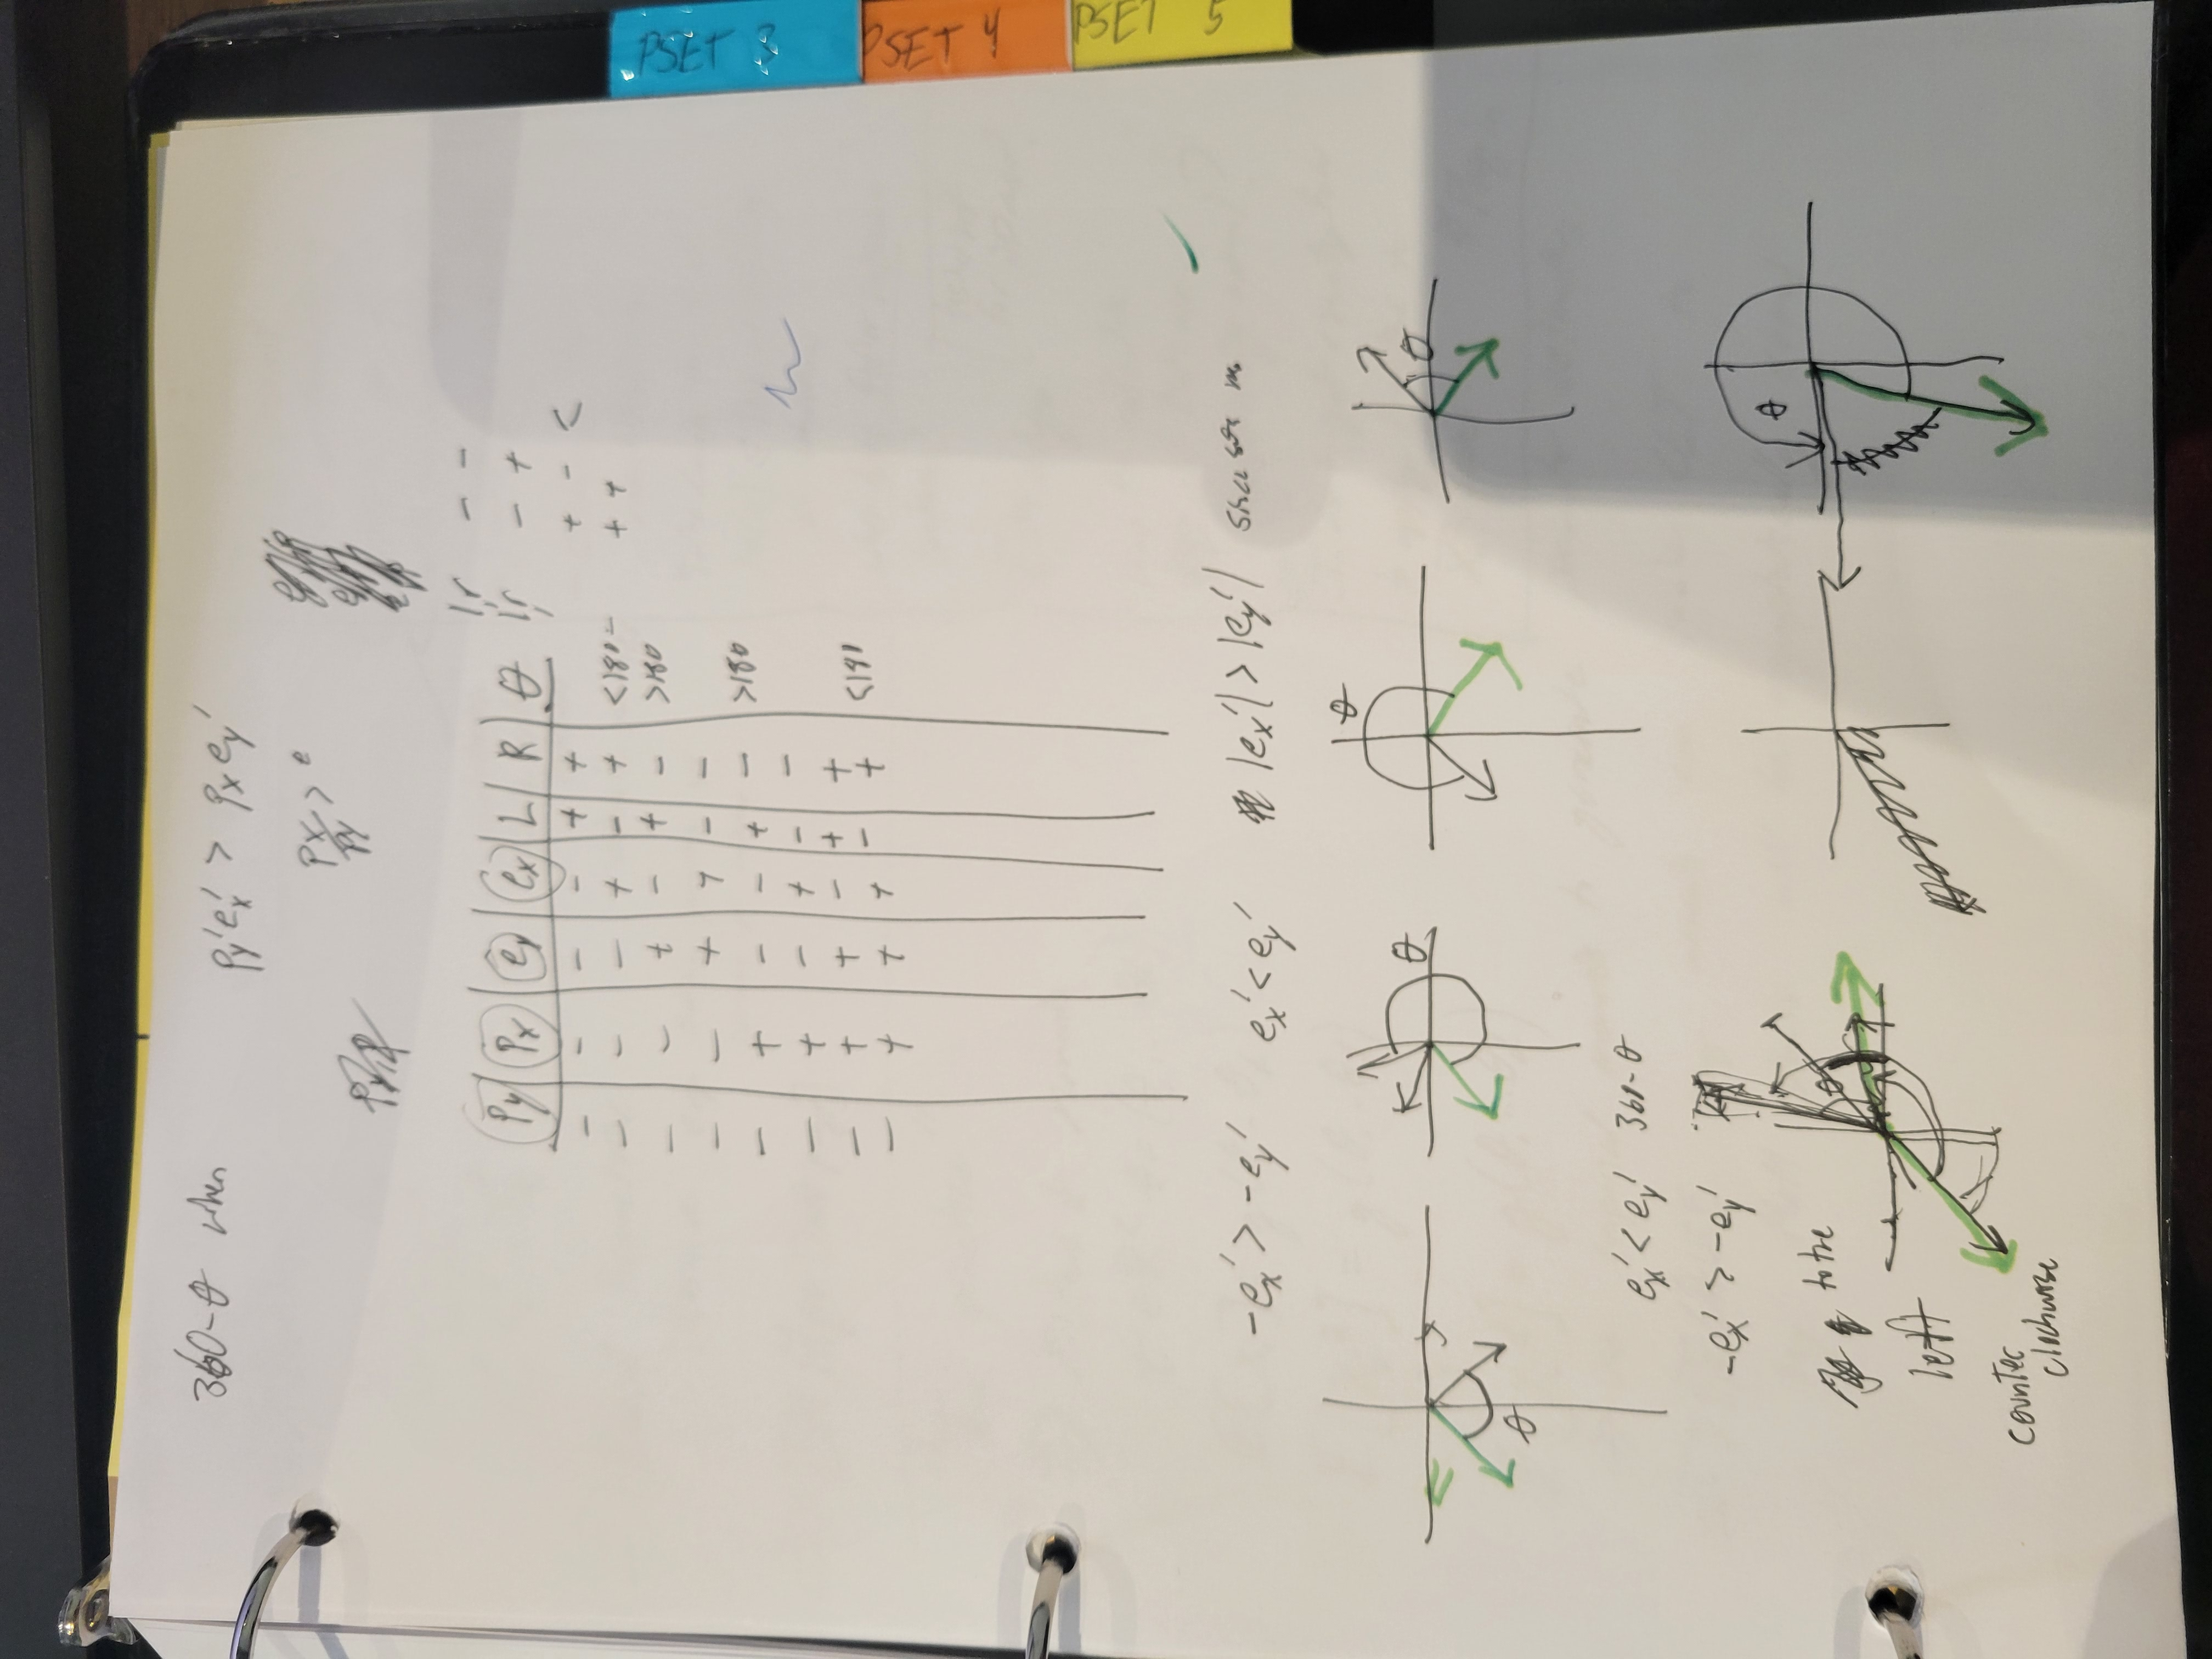
\includegraphics[width=0.9\textwidth]{Chapters/Postamble/appc_pics/phi_math_1.jpg}}       




   
\iffalse
    
            Derivation of infinite momentum frame Bjorken x. Take quark to have momentum fraction $\xi$ of proton's total momentum,i.e. $p_q = \xi p_2$:\\
            \indent Inf. Mom. frame - neglect proton mass so $p_2$ = $E_2$, neglect all transverse momenta:\\
            \indent Struck quark 4-momenta: $p_q = \xi p_2 = (\xi E_2, \xi E_2, 0, 0)$\\
            \indent 4-momenta of quark after interaction: $(p_q + q) = (\xi p_2 +q)$\\
            \indent Square the 4-momenta $(\xi p_2 +q)^2 = \xi^2 p_2^2 +q^2 + 2\xi p_2 \cdot q  = m_q^2$\\
            \indent Continue, noting $p_q = \xi p_2$ : $m_q^2 = p_q^2 - Q^2 + 2 \xi p_2 \cdot q$\\
            \indent Since $p_q^2$ = $m_q^2$, we have: $m_q^2 = m_q^2 -Q^2 + 2 \xi p_2 \cdot q$\\
            \indent So $0 = -Q^2 + 2\xi p_2 \cdot q \longrightarrow \xi = \frac{Q^2}{2 p_2 \cdot q} = x_B$\\

        \fi